\documentclass[aspectratio=169]{beamer}

\usepackage{natbib}
\usepackage{multirow}
\usepackage[linesnumbered,lined]{algorithm2e}

\usetheme{metropolis}
\setbeamercolor{background canvas}{bg=white}

\hypersetup{
    pdfauthor={Vineet John}, 
    colorlinks=true,
    linkcolor=black,
    citecolor=red,
    filecolor=magenta,
    urlcolor=cyan
}

% Custom commands
\newcommand{\imgsrc}[1]{\tiny{Source: #1}}
\newcommand{\loss}[1]{\mathcal{L}_{\text{#1}}}
\newcommand{\weight}[1]{\lambda_{\text{#1}}}
\newcommand{\param}[1]{\theta_{\text{#1}}}
\newcommand{\tabh}[1]{\multicolumn{1}{c|}{\textbf{#1}}}
\newcommand{\tabc}[2]{\multicolumn{1}{|c|}{\multirow{#1}{*}{\textbf{#2}}}}

% Title Slide
\title{
	Disentangled Representation Learning\\
	for Linguistic Style Transfer}
\date{}
\author{Vineet John}
\institute{University of Waterloo}

\begin{document}

\maketitle
\graphicspath{{images/}}

\section{Motivation}

\begin{frame}{Universal Function Approximators}
	\centering
	\begin{figure}[ht]
		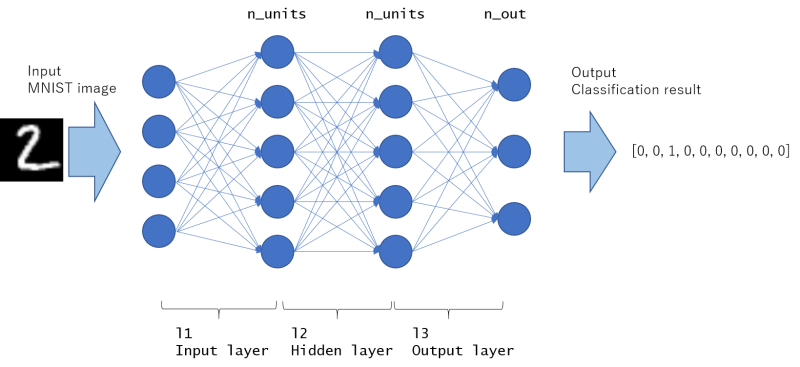
\includegraphics[width=\linewidth]{mlp-network}
	\end{figure}
	\imgsrc{\url{http://corochann.com/mnist-training-with-multi-layer-perceptron-1149.html}}
\end{frame}

\begin{frame}{Non-Interpretable Latent Representations}
	\begin{itemize}
		\item Neural networks can model arbitrarily complex functions.
		\item The initial set of parameters are set randomly.
		\item The learned parameters usually do not demonstrate a visible pattern.
	\end{itemize}
	$$f(x) + \epsilon = f'(x)$$
	\centering
	\begin{figure}[ht]
		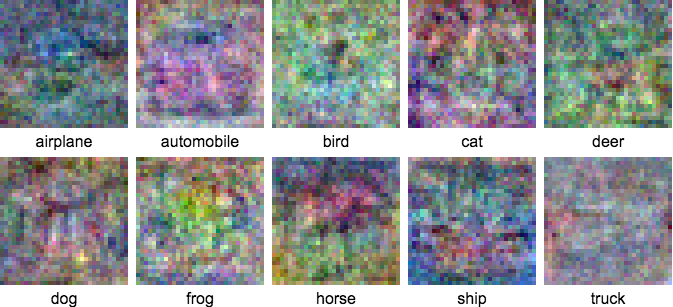
\includegraphics[width=0.5\linewidth]{uninterpretable-weights}
	\end{figure}
	\imgsrc{\url{https://ml4a.github.io/ml4a/looking_inside_neural_nets}}
\end{frame}

\begin{frame}{Style and Content in Language}
	\centering
	\LARGE
	\begin{table}[ht]
		\centering
		\begin{tabular}{ l  c | c | c | c | c |}
			\\
			\cline{3-6}
			I love this movie & $\rightarrow$ & $0.21$ & $0.32$ & $0.74$ & $0.43$ \\
			\cline{3-6}
			I hate this movie & $\rightarrow$ & $0.45$ & $0.78$ & $0.97$ & $0.17$ \\
			\cline{3-6}
		\end{tabular}
		\pause
		{\Huge$$\Downarrow$$}
		\begin{tabular}{ l  c | c | c | c | c |}
			\cline{3-6}
			I love this movie & $\rightarrow$ & $0.68$ & $0.12$ & $0.33$ & {\color{red}$1.00$} \\
			\cline{3-6}
			I hate this movie & $\rightarrow$ & $0.68$ & $0.12$ & $0.33$ & {\color{red}$0.00$} \\
			\cline{3-6}
		\end{tabular}
	\end{table}
\end{frame}

\begin{frame}{Style and Content in Language}
	The idea of style and content in language are vague and open to interpretation.

	However, most researchers in the NLP community use discrete or continuous attributes in text like
	\begin{itemize}
		\item Sentiment \citep{hu2017toward,shen2017style,fu2017style}
		\item Tense \citep{hu2017toward}
		\item Publication Medium \citep{fu2017style}
		\item Question Topic \citep{kim2017adversarially}
		\item Political Slant \citep{prabhumoye2018style}
	\end{itemize}
\end{frame}

\begin{frame}{Problem Statement}
	\centering
	\Huge{Disentangle the latent variables for \textbf{style} and \textbf{content} in language models, thereby learning interpretable sentence representations}
\end{frame}

\begin{frame}{Auxiliary Problem Statement}
	\centering
	\Huge{Generate \textbf{plausible sentences} in a user-defined style, while retaining the original content of the source sentences}
\end{frame}

% 

\section{Background}

\begin{frame}{Autoencoding}
	\centering
	\begin{figure}[ht]
		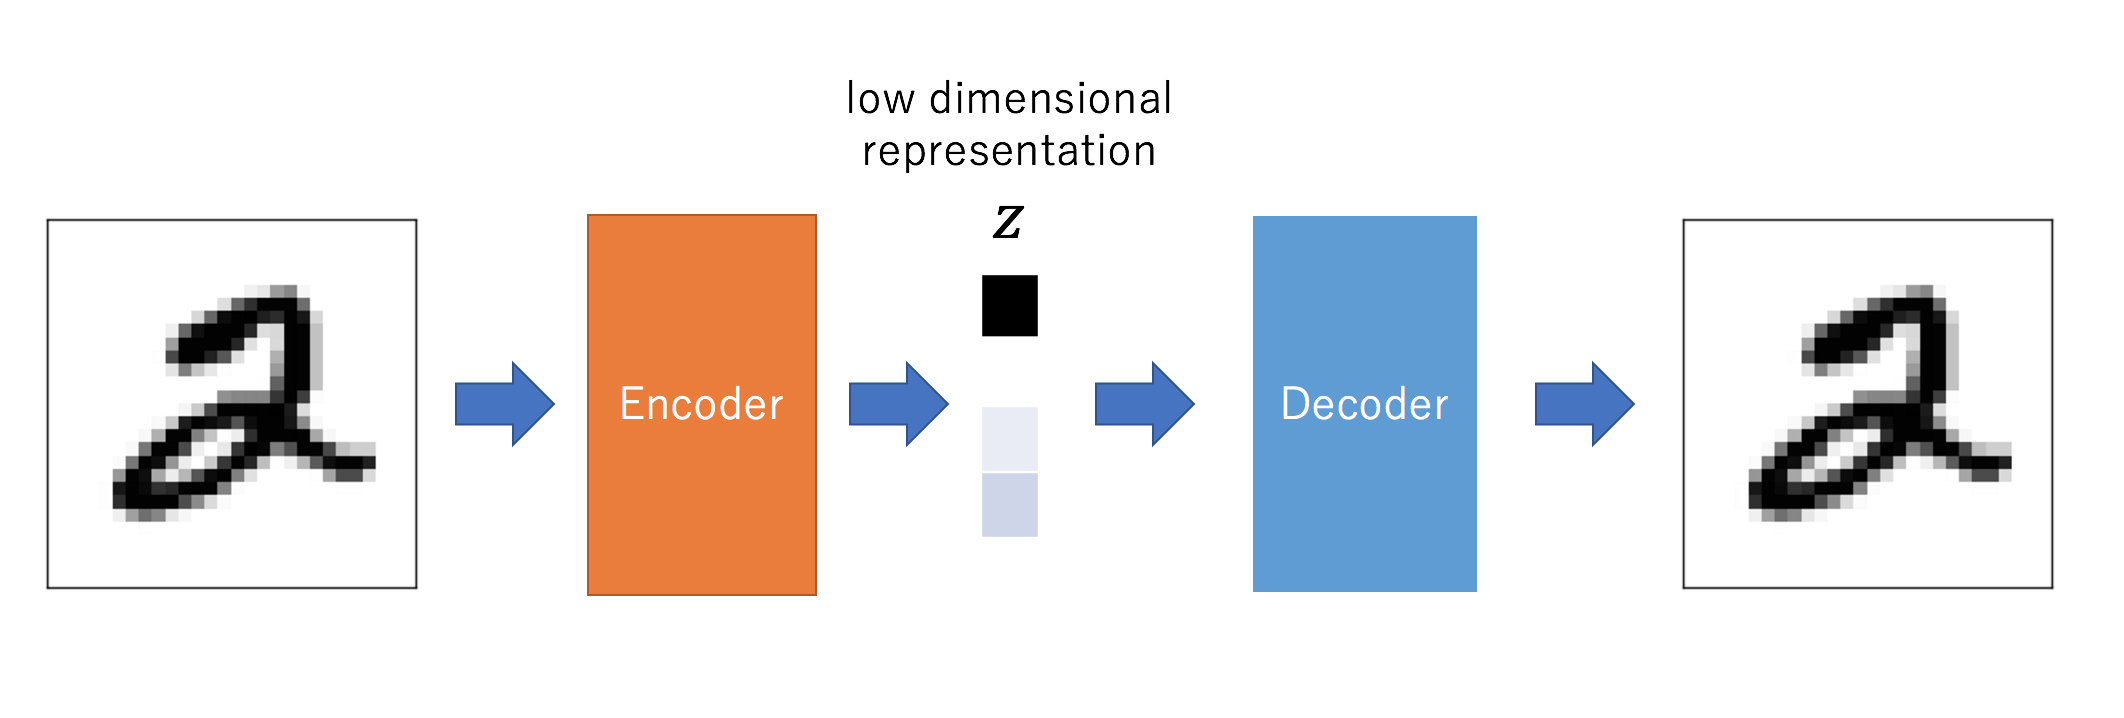
\includegraphics[width=\linewidth]{dae-structure}
	\end{figure}
	\imgsrc{\url{http://mlexplained.com/2017/12/28/an-intuitive-explanation-of-variational-autoencoders-vaes-part-1}}
\end{frame}

\begin{frame}{Variational Autoencoding}
	\centering
	\begin{figure}[ht]
		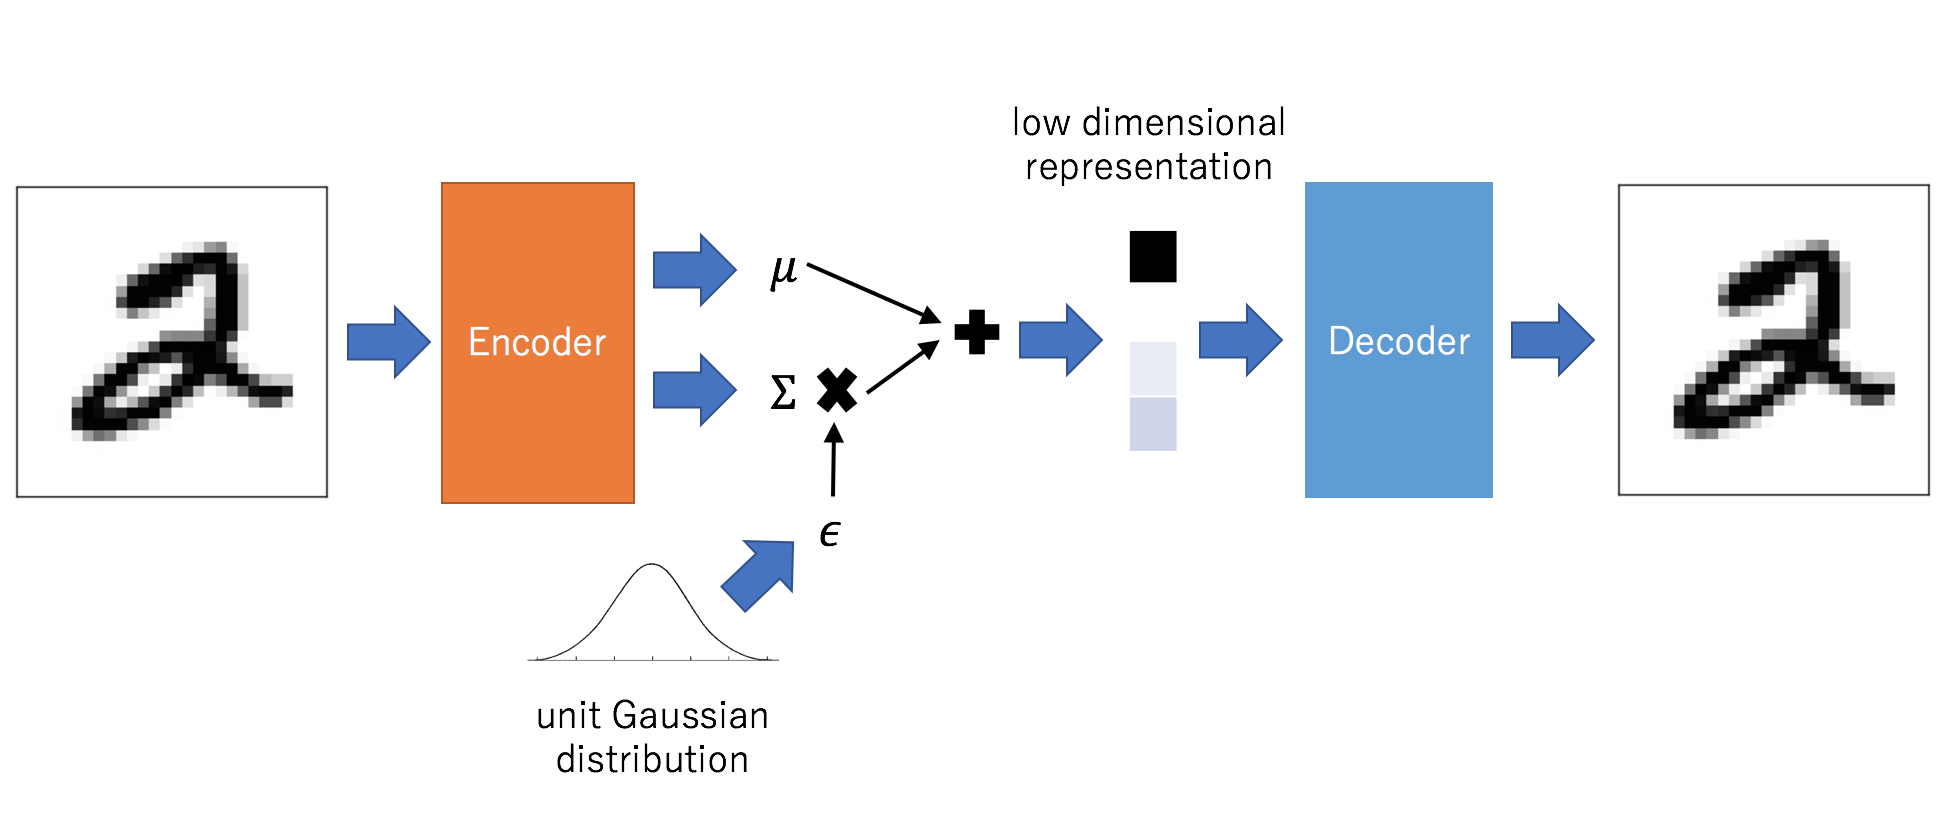
\includegraphics[width=\linewidth]{vae-structure}
	\end{figure}
	\imgsrc{\url{http://mlexplained.com/2017/12/28/an-intuitive-explanation-of-variational-autoencoders-vaes-part-1}}
\end{frame}

\begin{frame}{Sequence Autoencoding}
	\centering
	\begin{figure}[ht]
		\makeatletter
\ifx\du\undefined
  \newlength{\du}
\fi
\setlength{\du}{\unitlength}
\ifx\spacing\undefined
  \newlength{\spacing}
\fi
\setlength{\spacing}{60\unitlength}
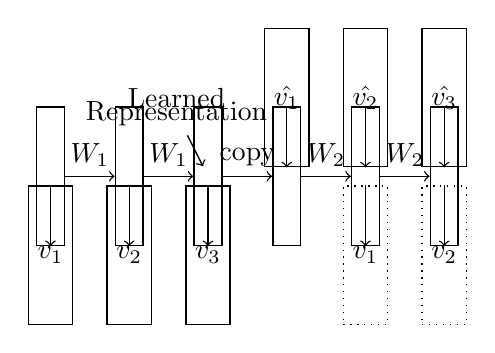
\begin{tikzpicture}
\pgfsetlinewidth{0.5\du}
\pgfsetmiterjoin
\pgfsetbuttcap

\node[rectangle, draw=black, minimum width=10\du, minimum height=50\du] (v1) at (0\spacing, 0) {$v_1$};
\node[rectangle, draw=black, minimum width=10\du, minimum height=50\du] (v2) at (\spacing, 0) {$v_2$};
\node[rectangle, draw=black, minimum width=10\du, minimum height=50\du] (v3) at (2\spacing, 0) {$v_3$};

\node[rectangle, dotted, draw=black, minimum width=10\du, minimum height=50\du] (v5) at (4\spacing, 0) {$v_1$};
\node[rectangle, dotted, draw=black, minimum width=10\du, minimum height=50\du] (v6) at (5\spacing, 0) {$v_2$};

\node[rectangle, draw=black, minimum width=10\du, minimum height=50\du] (h1) at (0\spacing, \spacing) {};
\node[rectangle, draw=black, minimum width=10\du, minimum height=50\du] (h2) at (\spacing, \spacing) {};
\node[rectangle, draw=black, minimum width=10\du, minimum height=50\du] (h3) at (2\spacing, \spacing) {};

\node[rectangle, draw=black, minimum width=10\du, minimum height=50\du] (h4) at (3\spacing, \spacing) {};
\node[rectangle, draw=black, minimum width=10\du, minimum height=50\du] (h5) at (4\spacing, \spacing) {};
\node[rectangle, draw=black, minimum width=10\du, minimum height=50\du] (h6) at (5\spacing, \spacing) {};

\node[rectangle, draw=black, minimum width=10\du, minimum height=50\du] (v4r) at (3\spacing, 2\spacing) {$\hat{v_1}$};
\node[rectangle, draw=black, minimum width=10\du, minimum height=50\du] (v5r) at (4\spacing, 2\spacing) {$\hat{v_2}$};
\node[rectangle, draw=black, minimum width=10\du, minimum height=50\du] (v6r) at (5\spacing, 2\spacing) {$\hat{v_3}$};

\node[anchor=center]  at (1.6\spacing, 2\spacing) {Learned};
\node[anchor=center] (p1) at (1.6\spacing, 1.8\spacing) {Representation};
\node[anchor=center] (p2) at (2\spacing, \spacing) {};
%\node[anchor=center] (w) at (0\spacing, 0.5\spacing) {$\WW_1$};

%\draw[ultra thick, ->] (2aa) -- node[left] {Conv Net} (3a);
\draw[->] (v1) -- (h1);
\draw[->] (v2) -- (h2);
\draw[->] (v3) -- (h3);
\draw[->] (v5) -- (h5);
\draw[->] (v6) -- (h6);

\draw[->] (h1) -- node[above] {$W_1$} (h2);
\draw[->] (h2) -- node[above] {$W_1$} (h3);
\draw[->] (h3) -- node[above] {copy} (h4);
\draw[->] (h4) -- node[above] {$W_2$} (h5);
\draw[->] (h5) -- node[above] {$W_2$} (h6);

\draw[->] (h4) -- (v4r);
\draw[->] (h5) -- (v5r);
\draw[->] (h6) -- (v6r);

\draw[->] (p1) -- (p2);
\end{tikzpicture}

	\end{figure}
	\imgsrc{\citet{srivastava2015unsupervised}}
\end{frame}

\begin{frame}{Multi-Task Learning}
	Augmenting the holistic objective with an auxiliary objective to improve the learned representations.

	Multi-task losses are used in previous work for:
	\begin{itemize}
		\item Sequence-to-sequence learning \citep{luong2015multi}
		\item Sentence representation learning \citep{jernite2017discourse}
		\item Sentiment analysis \citep{balikas2017multitask}
	\end{itemize}
\end{frame}

\begin{frame}{Adversarial Learning}
	Specialized case of multi-task learning to provide a negative signal as a regularizer to a generative network.

	\centering
	\begin{figure}[ht]
		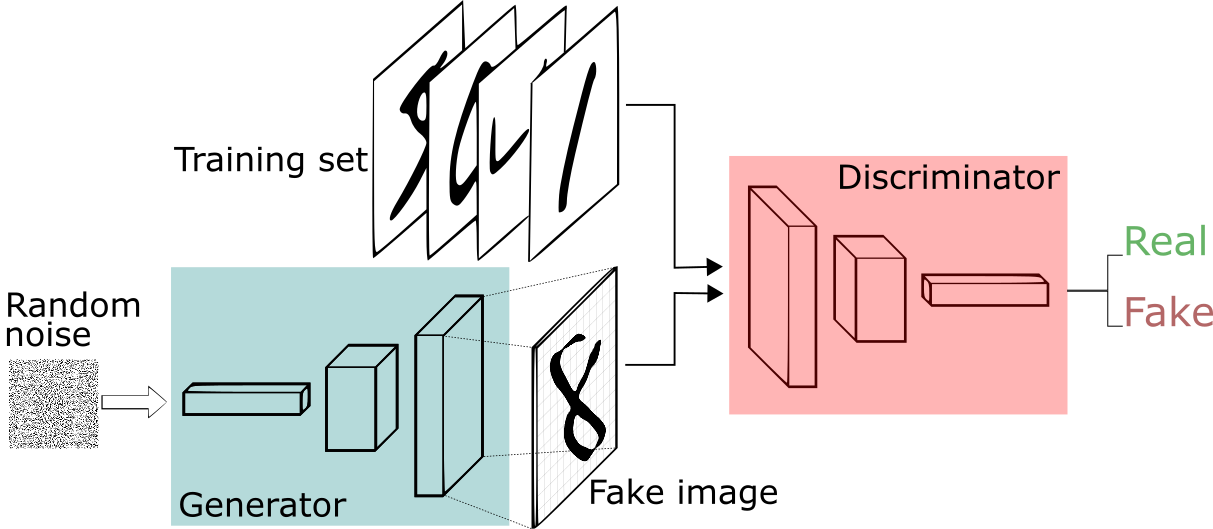
\includegraphics[width=0.8\textwidth]{images/gans}
	\end{figure}
	\imgsrc{\url{https://deeplearning4j.org/generative-adversarial-network}}
\end{frame}

\begin{frame}{Visual Style Transfer}
	\centering
	(a) Content, (b) Style and (c) Synthesized Images
	\begin{figure}[ht]
		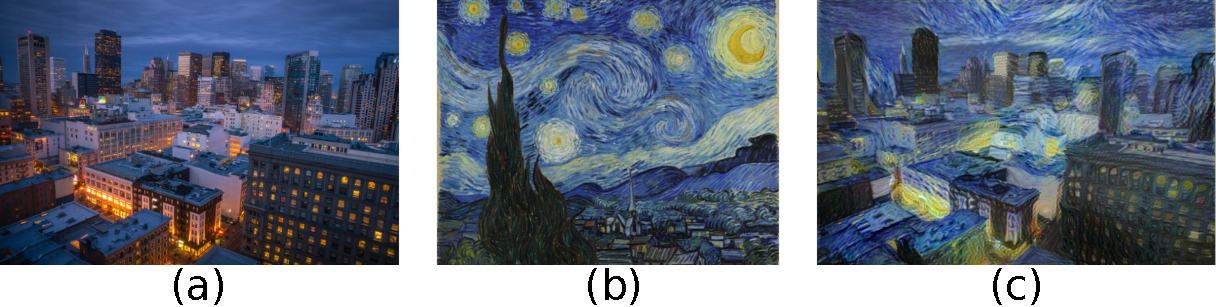
\includegraphics[width=\textwidth]{images/style-transfer-vision}
	\end{figure}
	\imgsrc{\url{https://github.com/fzliu/style-transfer}}
\end{frame}

% 

\section{Approach}

\begin{frame}{Sequence Autoencoder}
	\centering
	\begin{figure}[ht]
		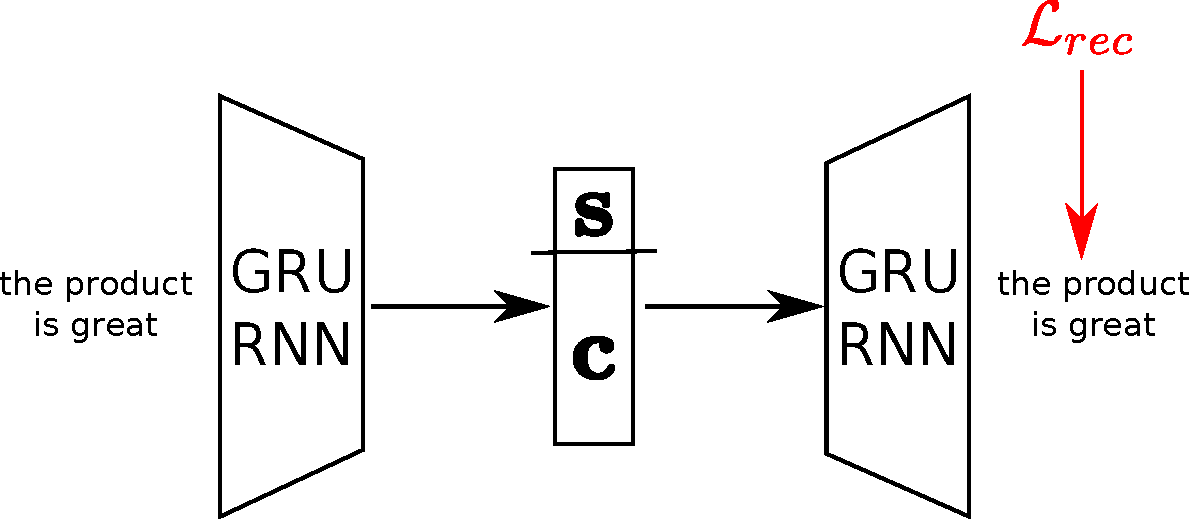
\includegraphics[width=\textwidth]{images/overview-training-1}
	\end{figure}
\end{frame}

\begin{frame}{Sequence Autoencoder - Deterministic}
	\textbf{Minimize the negative log-likelihood} of each predicted word, given the previous words.
	\begin{equation} \label{eqn:dae-rec}
		\loss{rec}(\param{E},\param{D}; x) = - \sum_{t=1}^T \log p(x_t | h_t, x_1, x_2 \cdots, x_{t-1})
	\end{equation}
	where $x_1, x_2 \cdots$ are the features for each word \citep{mikolov2013distributed,pennington2014glove}, and $h_t = [s_t; c_t]$ is the final hidden state of the encoder.

	Trained using a \textbf{sequence cross-entropy loss}, we use the average cross-entropy per time-step to train the model.
	\begin{equation*}
		\mathcal{H}_{x'} (x) = - \sum_{i}^V x_{i}' \log (x_i)
	\end{equation*}
	where $V$ is the size of the vocabulary, $x'$ and $x$ are the true and predicted distributions respectively.
\end{frame}

\begin{frame}{Sequence Autoencoder - Variational}
	The probabilistic sampling and KL divergence losses are applied for both the style space $s$ and the content space $c$, separately. The weights applied to each KL divergence loss are tuned independently as a hyperparameter.

	\begin{align} \label{eqn:vae-rec}
		\loss{rec}(\param{E},\param{D}; x) =
		 & - \mathbb{E}_{q_{E}(s|x) q_{E}(c|x)} [\log p_D(x|s,c)] \nonumber \\
		 & + \weight{skl} KL(q_{E}(s|x)||p(z))                    \nonumber \\
		 & + \weight{ckl} KL(q_{E}(c|x)||p(z))
	\end{align}
\end{frame}

\begin{frame}{Multi-Task Style Classifier}
	\centering
	\begin{figure}[ht]
		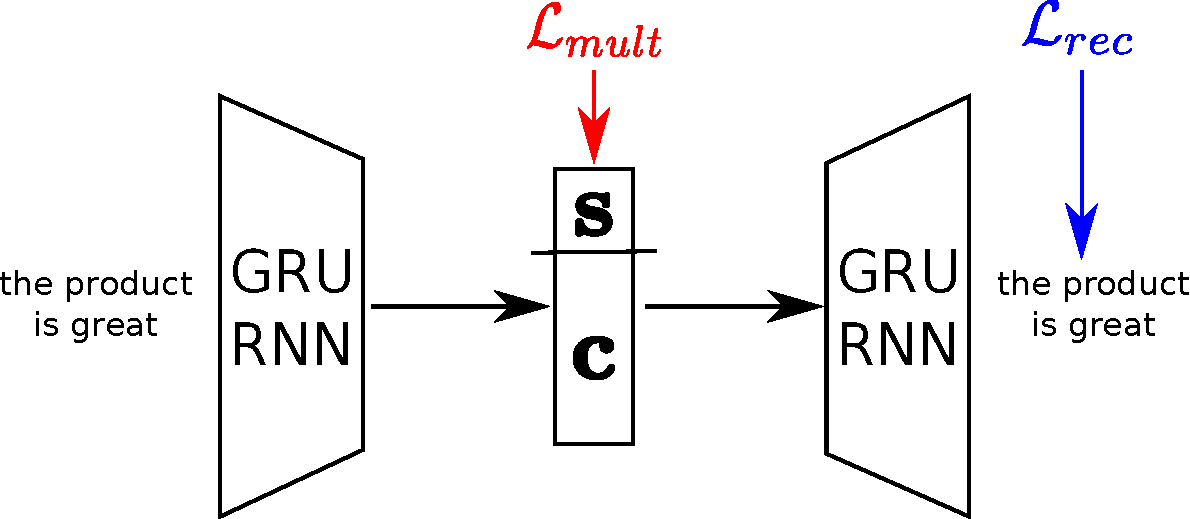
\includegraphics[width=\textwidth]{images/overview-training-2}
	\end{figure}
\end{frame}

\begin{frame}{Multi-Task Style Classifier}
	We use a simple multi-layer perceptron (MLP) followed by a softmax distribution over the possible labels

	\begin{equation} \label{eqn:multi-task-loss}
		\loss{mult}(\param{E};\param{mult}) = - \mathbb{E} [\log p(y|s;\param{mult})]
	\end{equation}
	where $\param{mult}$ are the classifier's parameters for multi-task learning, and $y$ is the true label distribution.
\end{frame}

\begin{frame}{Style Discriminator}
	\centering
	\begin{figure}[ht]
		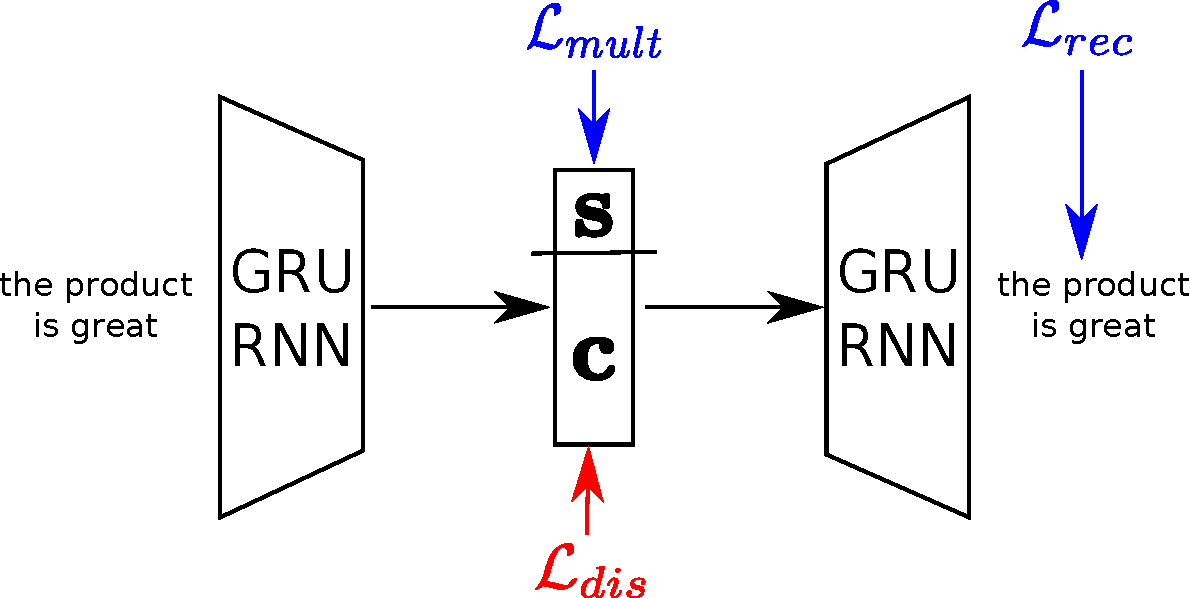
\includegraphics[width=\textwidth]{images/overview-training-3}
	\end{figure}
\end{frame}

\begin{frame}{Style Discriminator}
	\textbf{Discriminator Loss:}
	Given a set of pairs of features $x$ and labels $y$ in pairs $(x_n, y_n)$, we train a classifier that minimizes the negative log-likelihood of the predicted softmax distribution over the predicted labels.
	\begin{equation}
		\loss{dis}(\param{dis}) = - \mathbb{E} [\log p(y|c;\param{dis})]
	\end{equation}
	where $y$ is the true label distribution.

	\textbf{Adversarial Loss:}
	The adversarial loss applied to the autoencoder is the Shannon entropy of the predicted distribution.
	\begin{equation}
		\loss{adv}(\param{E}) = - \mathcal{H}(p_\text{dis}(y|c))
	\end{equation}
\end{frame}

\begin{frame}{Content Discriminator}
	\centering
	\begin{figure}[ht]
		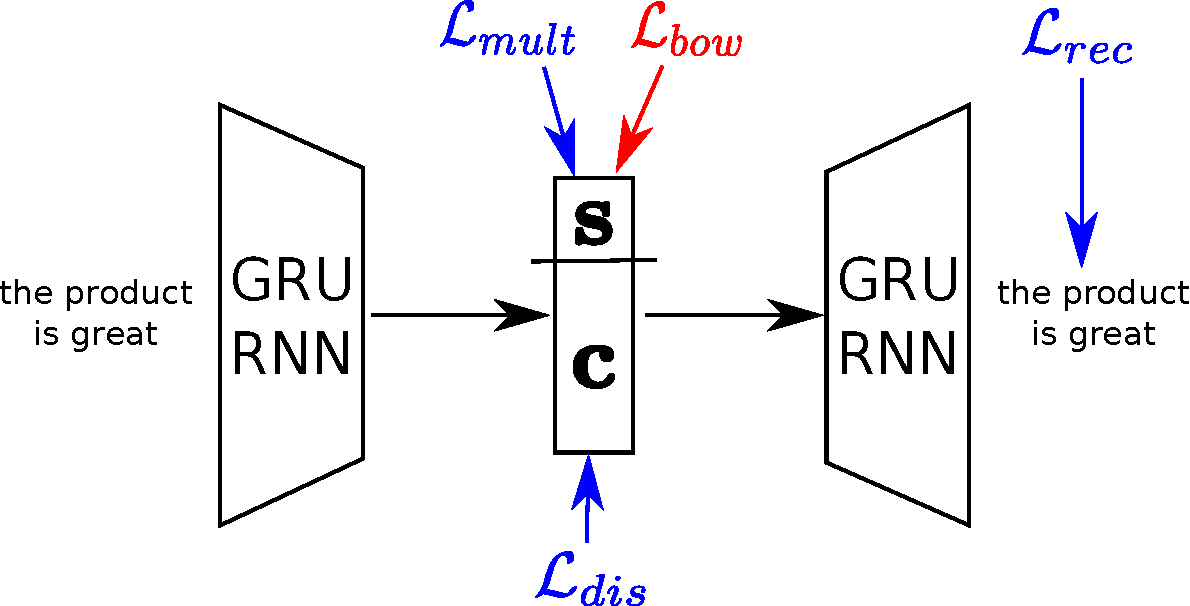
\includegraphics[width=\textwidth]{images/overview-training-4}
	\end{figure}
\end{frame}

\begin{frame}{Content Discriminator}
	\textbf{Discriminator Loss:}
	Given the corpus of sentences, and their bag-of-words representations, we train a bag-of-words classifier that minimizes the negative log-likelihood of the predicted softmax distribution over the predicted vocabulary.
	\begin{equation} \label{eqn:bow-disc-loss}
		\loss{bow}(\param{bow}) = - \mathbb{E} [\log p(b|c;\param{bow})]
	\end{equation}

	\textbf{Adversarial Loss:}
	The adversarial loss applied to the autoencoder is the Shannon entropy of the predicted distribution.
	\begin{equation}
		\loss{badv}(\param{E}) = - \mathcal{H}(p_\text{bow}(b|c))
	\end{equation}
\end{frame}

\begin{frame}{Model Training}
	\centering
	\begin{figure}[ht]
		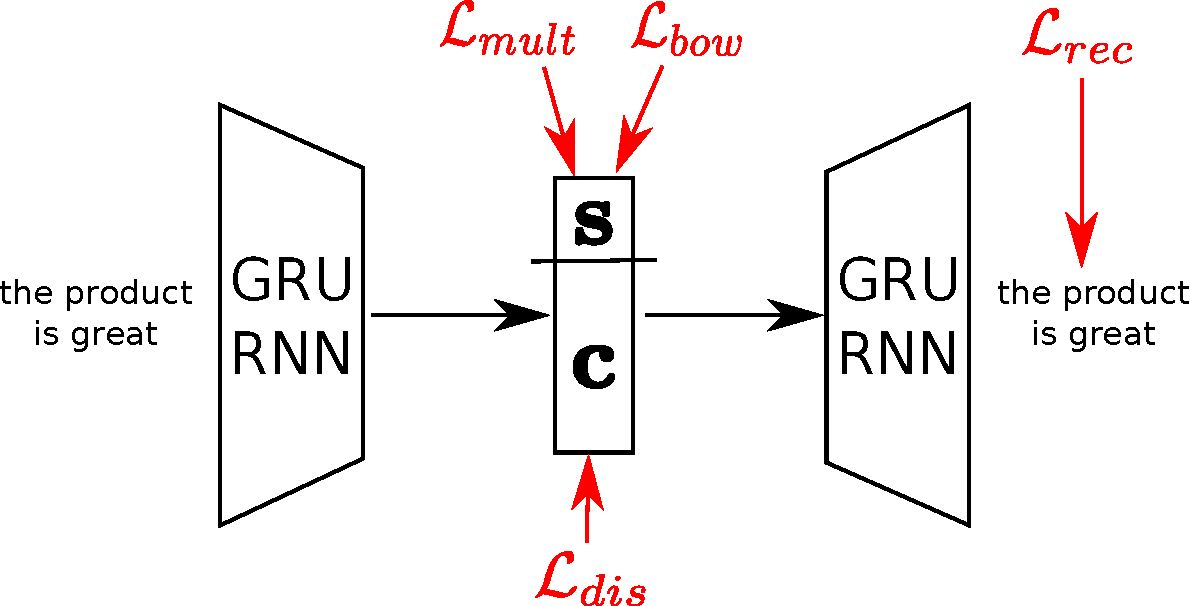
\includegraphics[width=\textwidth]{images/overview-training-all}
	\end{figure}
\end{frame}

\begin{frame}{Model Training}
	\textbf{Overall Autoencoder Model Loss:}
	\begin{align*}
		\loss{ovr} =
		 & \loss{rec}(\param{E},\param{D}) + \weight{mult} \loss{mult} (\param{E},\param{mult}) \\
		 & - \weight{adv} \loss{adv}(\param{E}) - \weight{badv} \loss{badv}(\param{E})
	\end{align*}

	\textbf{Training Algorithm:}

	\centering
	\begin{minipage}{.7\linewidth}

		\begin{algorithm}[H]
			\While{epochs remaining}{
				minimize $\loss{dis}$ w.r.t. $\param{dis}$\;
				minimize $\loss{bow}$ w.r.t. $\param{bow}$\;
				minimize $\loss{ovr}$ w.r.t. $\param{E}, \param{D}, \param{mult}$\;
			}
		\end{algorithm}
	\end{minipage}
\end{frame}

\begin{frame}{Model Inference}
	\centering
	\begin{figure}[ht]
		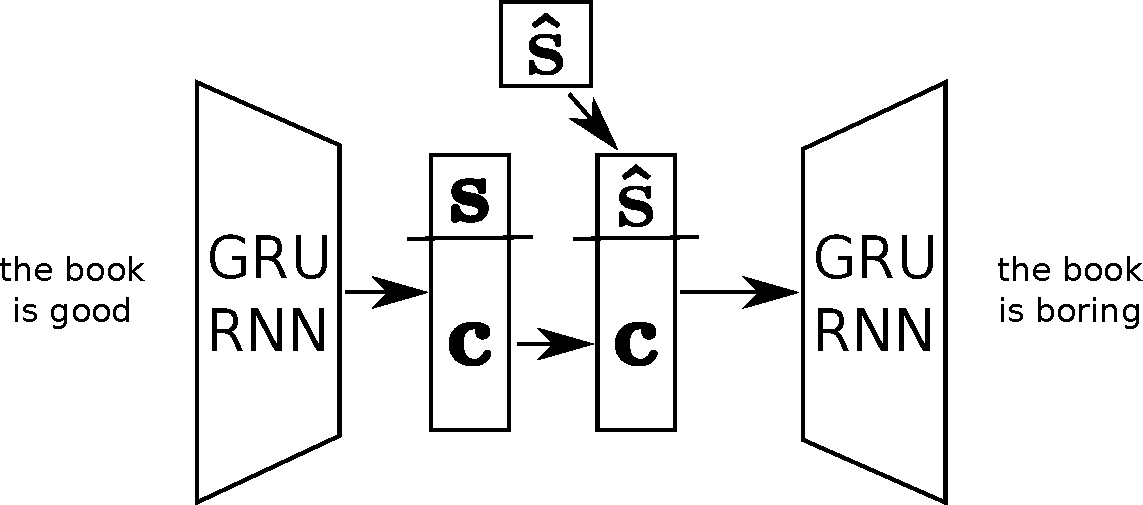
\includegraphics[width=\textwidth]{images/overview-inference}
	\end{figure}
\end{frame}

% 

\section{Datasets}

\begin{frame}{Datasets}
	\begin{columns}[T] % align columns
		\begin{column}{.48\textwidth}
			\Large
			\textbf{Yelp Service Reviews:}
			\begin{itemize}
				\item Train / Validation / Test = $444101$ / $126670$ / $63483$
				\item Max Sentence Length $= 15$
				\item Vocabulary Size $\approx 9200$
			\end{itemize}
		\end{column}
		\hfill
		\begin{column}{.48\textwidth}
			\Large
			\textbf{Amazon Product Reviews:}
			\begin{itemize}
				\item Train / Validation / Test = $559142$ / $2000$ / $2000$
				\item Max Sentence Length $= 20$
				\item Vocabulary Size $\approx 58000$
			\end{itemize}
		\end{column}
	\end{columns}

\end{frame}

\section{Evaluation Metrics}

\begin{frame}{Style Transfer Strength}

	The style transfer strength is the ratio of sentences successfully transferred to the target style, to the total number of test sentences, as predicted by a pre-trained CNN text classifier \citep{kim2014convolutional}.

	It is given by the following equation,
	\begin{equation*}
		\frac{\sum_{i=1}^{N}{(1 | y_i = y^*)}}{N}
	\end{equation*}
	where $N$ is the total number of generated sentences, $y*$ is the style attribute we wish to transfer, and $y_{1, 2 \cdots n}$ are the actual attributes as predicted by the pre-trained classifier.
\end{frame}

\begin{frame}{Content Preservation}
	Let $W$ be the set of word embeddings in any sentence $s$.

	Then the cosine similarity between two sentences $s_1$ and $s_2$ is obtained by
	\begin{align*}
		\text{emb} =    & [min(W);max(W);mean(W)]              \\
		\text{cossim} = & 1 - \cos(\text{emb}_1, \text{emb}_2)
	\end{align*}
	where $\text{emb}_1$ and $\text{emb}_2$ are the sentence embeddings for $s_1$ and $s_2$ respectively.

	The mean cosine similarity of all the sentences in the test dataset is reported as the content preservation.
\end{frame}

\begin{frame}{Word Overlap}
	Given a source sentence $x$ and an attribute style transferred sentence $y$, let $w_x$ and $w_y$ be the set of unique words present in $x$ and $y$ respectively.

	Then, the word overlap score can be calculated using
	\begin{equation*}
		\frac{count(w_x \cap w_y)}{count(w_x \cup w_y)}
	\end{equation*}
	which is simply a normalized measure of overlapping unigrams in the source and target.
\end{frame}

\begin{frame}{Language Fluency}
	We use a trigram based Kneser–Ney Smoothed language model \citep{kneser1995improved} as a quantifiable and automated scoring metric by which to assess the quality of generated sentences.

	\begin{equation*}
		\sum_{t=1}^T \log p(x_t | x_{t-1}, x_{t-2})
	\end{equation*}

	The log-likelihood is reported as a measure of language fluency.
\end{frame}

% 

\section{Results and Analysis}

\begin{frame}{Latent Space Classification}
	\begin{table}[ht]
		\centering
		\begin{tabular}{| l | r | r |}
			\hline
			                                & \tabh{DAE}                  & \tabh{VAE} \\
			\hline \hline
			Random/Majority guess           & \multicolumn{2}{c|}{0.6018}              \\ \hline \hline
			Content latent space  ($c$)     & 0.6137                      & 0.6567     \\ \hline
			Style latent space ($s$)        & 0.7927                      & 0.7911     \\ \hline
			Complete latent space ($[s;c]$) & 0.7918                      & 0.7918     \\
			\hline
		\end{tabular}
		\caption{Results - Style Classification Accuracy}
		\label{tab:latent-space-classification}
	\end{table}
\end{frame}

\begin{frame}{Ablation Tests}
	\begin{table}[ht]
		\centering
		\begin{tabular}{| l | r | r | r | r |}
			\hline
			\tabc{2}{Objectives}                                     & \tabh{Transfer} & \tabh{Content}      & \tabh{Word}     & \tabh{Language}   \\
			                                                         & \tabh{Strength} & \tabh{Preservation} & \tabh{Overlap}  & \tabh{Fluency}    \\
			\hline
			\hline
			$\loss{rec}$                                             & 0.1436          & \textbf{0.9154}     & \textbf{0.3288} & -14.2781          \\
			\hline
			$\loss{rec}$, $\loss{adv}$                               & 0.7274          & 0.8800              & 0.2037          & -14.1567          \\
			\hline
			$\loss{rec}$, $\loss{mult}$                              & 0.7894          & 0.8976              & 0.2589          & -14.5607          \\
			\hline
			$\loss{rec}$, $\loss{badv}$                              & 0.1677          & 0.9147              & 0.3282          & -14.4486          \\
			\hline
			$\loss{rec}$, $\loss{adv}$, $\loss{mult}$                & \textbf{0.8903} & 0.8824              & 0.2105          & -14.4099          \\
			\hline
			$\loss{rec}$, $\loss{adv}$, $\loss{badv}$                & 0.7491          & 0.8827              & 0.2022          & -14.3568          \\
			\hline
			$\loss{rec}$, $\loss{mult}$, $\loss{badv}$               & 0.7832          & 0.8958              & 0.2567          & -14.3373          \\
			\hline
			$\loss{rec}$, $\loss{adv}$, $\loss{mult}$, $\loss{badv}$ & 0.8846          & 0.8782              & 0.1970          & \textbf{-14.0479} \\
			\hline
		\end{tabular}
		\caption{Results - Ablation Tests}
		\label{tab:ablation-results}
	\end{table}
\end{frame}

\begin{frame}{Latent Space t-SNE plots}
	\centering
	\textbf{Deterministic Autoencoder}

	\begin{figure}[ht]
		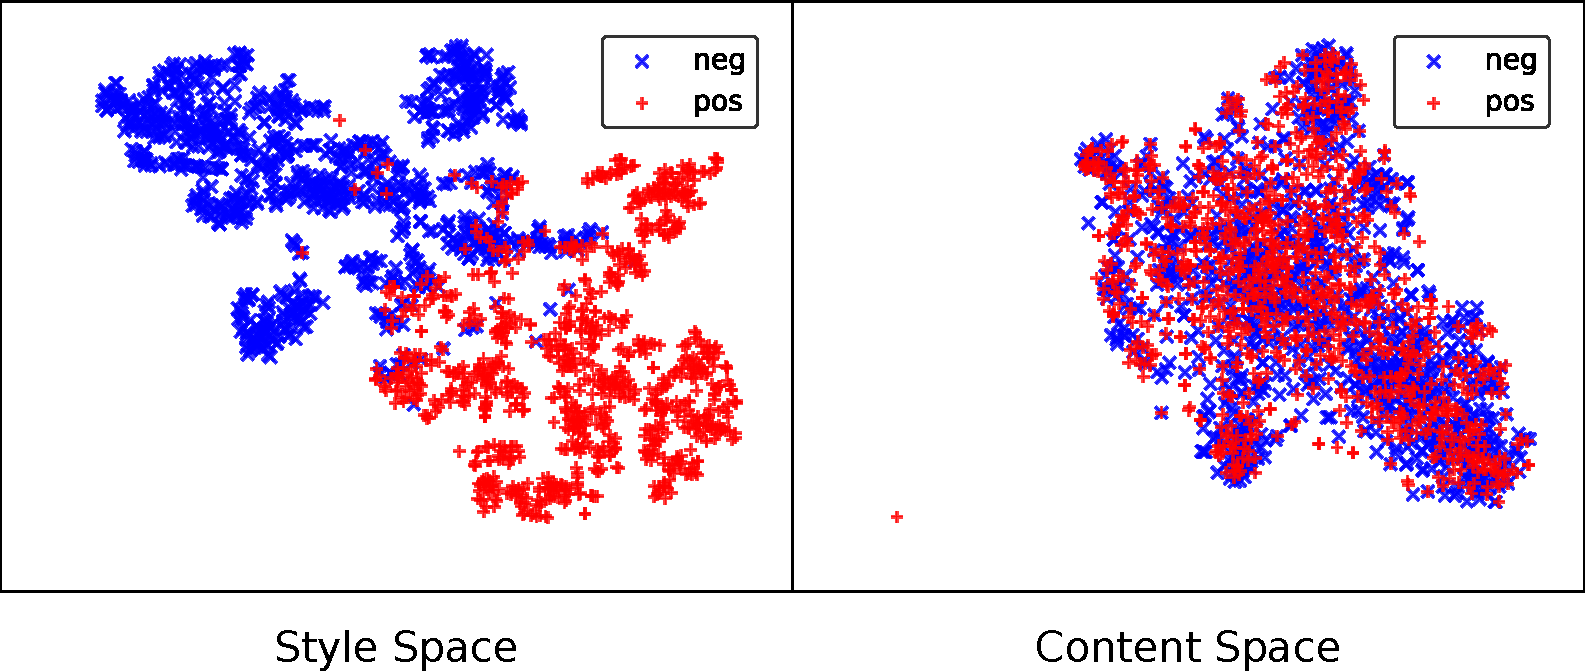
\includegraphics[width=\textwidth]{images/dae-latent-spaces}
	\end{figure}
\end{frame}

\begin{frame}{Latent Space t-SNE plots}
	\centering
	\textbf{Variational Autoencoder}

	\begin{figure}[ht]
		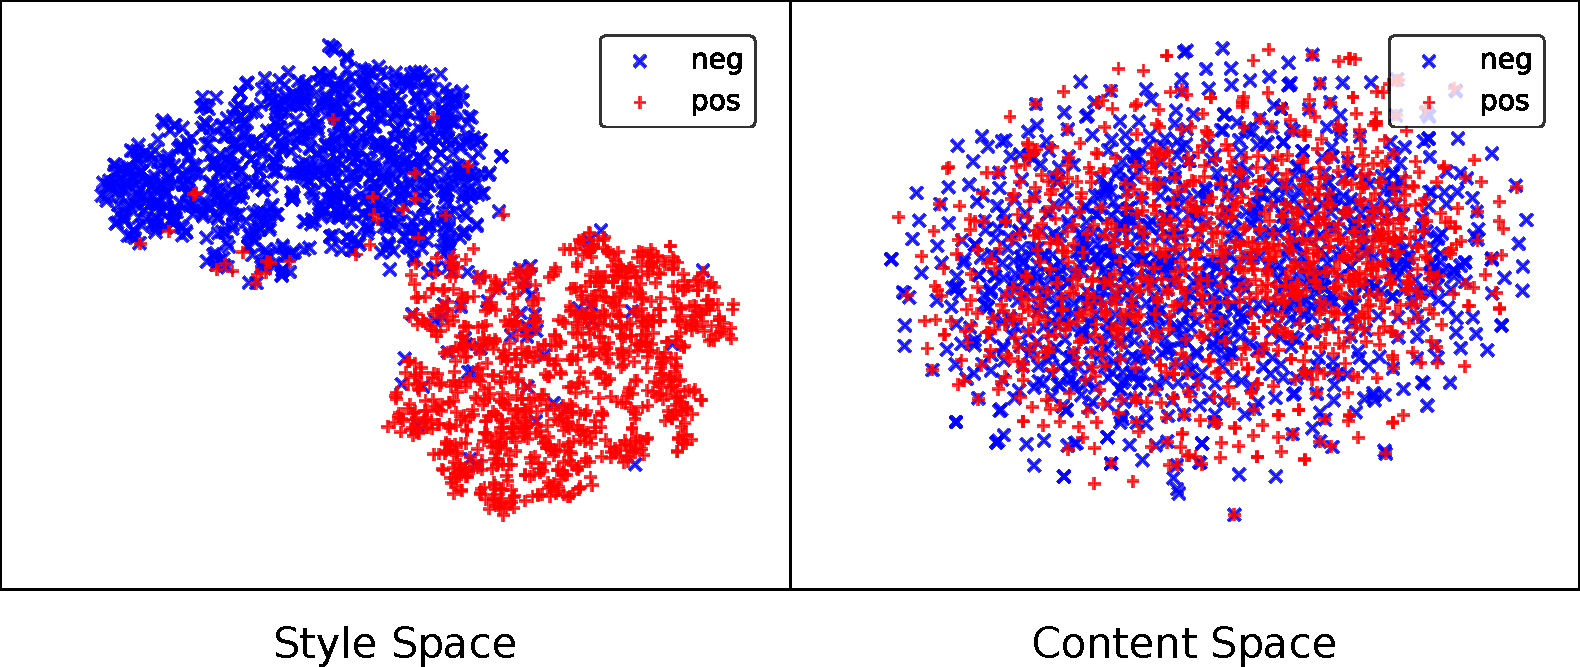
\includegraphics[width=\textwidth]{images/vae-latent-spaces}
	\end{figure}
\end{frame}

\begin{frame}{Style Transfer Results - Yelp}
	\begin{table}[ht]
		\centering
		\begin{tabular}{| l | r | r | r | r |}
			\hline
			\tabc{2}{Model}                       & \tabh{Transfer} & \tabh{Content}      & \tabh{Word}    & \tabh{Language} \\
			                                      & \tabh{Strength} & \tabh{Preservation} & \tabh{Overlap} & \tabh{Fluency}  \\
			\hline
			\hline
			Cross-Alignment \citep{shen2017style} & 0.8087          & 0.8920              & 0.2087         & -23.3886        \\
			\hline
			Style Embedding \citep{fu2017style}   & 0.1819          & 0.9586              & 0.6661         & -16.1711        \\
			\hline
			Ours (DAE)                            & 0.8425          & 0.8924              & 0.2552         & -16.4808        \\
			\hline
			Ours (VAE)                            & 0.8903          & 0.8824              & 0.2105         & -14.4099        \\
			\hline
		\end{tabular}
		\caption{Results - Yelp Dataset Sentiment Transfer}
		\label{tab:comparison-previous}
	\end{table}
\end{frame}

\begin{frame}{Style Transfer Results - Amazon}
	\begin{table}[ht]
		\centering
		\begin{tabular}{| l | r | r | r | r |}
			\hline
			\tabc{2}{Model}                       & \tabh{Transfer} & \tabh{Content}      & \tabh{Word}    & \tabh{Language} \\
			                                      & \tabh{Strength} & \tabh{Preservation} & \tabh{Overlap} & \tabh{Fluency}  \\
			\hline
			\hline
			Cross-Alignment \citep{shen2017style} & 0.6063          & 0.8933              & 0.0241         & -26.3093        \\
			\hline
			Style Embedding \citep{fu2017style}   & 0.4165          & 0.9332              & 0.3588         & -28.1346        \\
			\hline
			Ours (DAE)                            & 0.7032          & 0.9178              & 0.1305         & -32.4184        \\
			\hline
			Ours (VAE)                            & 0.7259          & 0.9090              & 0.0814         & -28.4953        \\
			\hline
		\end{tabular}
		\caption{Results - Amazon Dataset Sentiment Transfer}
		\label{tab:comparison-previous-ama}
	\end{table}
\end{frame}

\begin{frame}{Examples of Style Transfer}
	\centering
	\begin{table}[ht]
		\centering
		\begin{tabular}{| p{0.3\linewidth} | p{0.3\linewidth} | p{0.3\linewidth} |}
			\hline
			\tabc{2}{Original (Positive)}                    & \tabh{DAE Transferred}                                & \tabh{VAE Transferred}                             \\
			                                                 & \tabh{(Negative)}                                     & \tabh{(Negative)}                                  \\
			\hline
			\hline
			i would recommend a visit here                   & i would not recommend this place again                & i would not recommend this place for my experience \\
			\hline
			the restaurant itself is romantic and quiet      & the restaurant itself is soooo quiet                  & the restaurant itself was dirty                    \\
			\hline
			the food is very very amazing like beef and fish & the food is very horrible i have ever had mostly fish & the food is very bland and just not fresh          \\
			\hline
			we will definitely come back here                & we will not come back here again                      & we will never come back here                       \\
			\hline
		\end{tabular}
	\end{table}
\end{frame}

\begin{frame}{Examples of Style Transfer}
	\centering
	\begin{table}[ht]
		\centering
		\begin{tabular}{| p{0.3\linewidth} | p{0.3\linewidth} | p{0.3\linewidth} |}
			\hline
			\tabc{2}{Original (Negative)}                          & \tabh{DAE Transferred}                                & \tabh{VAE Transferred}                                      \\
			                                                       & \tabh{(Positive)}                                     & \tabh{(Positive)}                                           \\
			\hline
			\hline
			crap fries hard hamburger buns burger tasted like crap & cheap and yummy sandwiches really something different & yummy hamburgers and blue cheese bagels are classic italian \\
			\hline
			oh and terrible tea                                    & oh and awesome tea                                    & oh and great tea                                            \\
			\hline
			the interior is old and generally falling apart        & the interior is clean and orderly as entertaining     & the interior is old and noble                               \\
			\hline
			the crust was kinda gooey like                         & the crust is kinda traditional                        & the crust is soooooo worth it                               \\
			\hline
		\end{tabular}
	\end{table}
\end{frame}

% 

\section{Related Work}

\begin{frame}{Controlled Text Generation}
	\centering
	\begin{figure}[ht]
		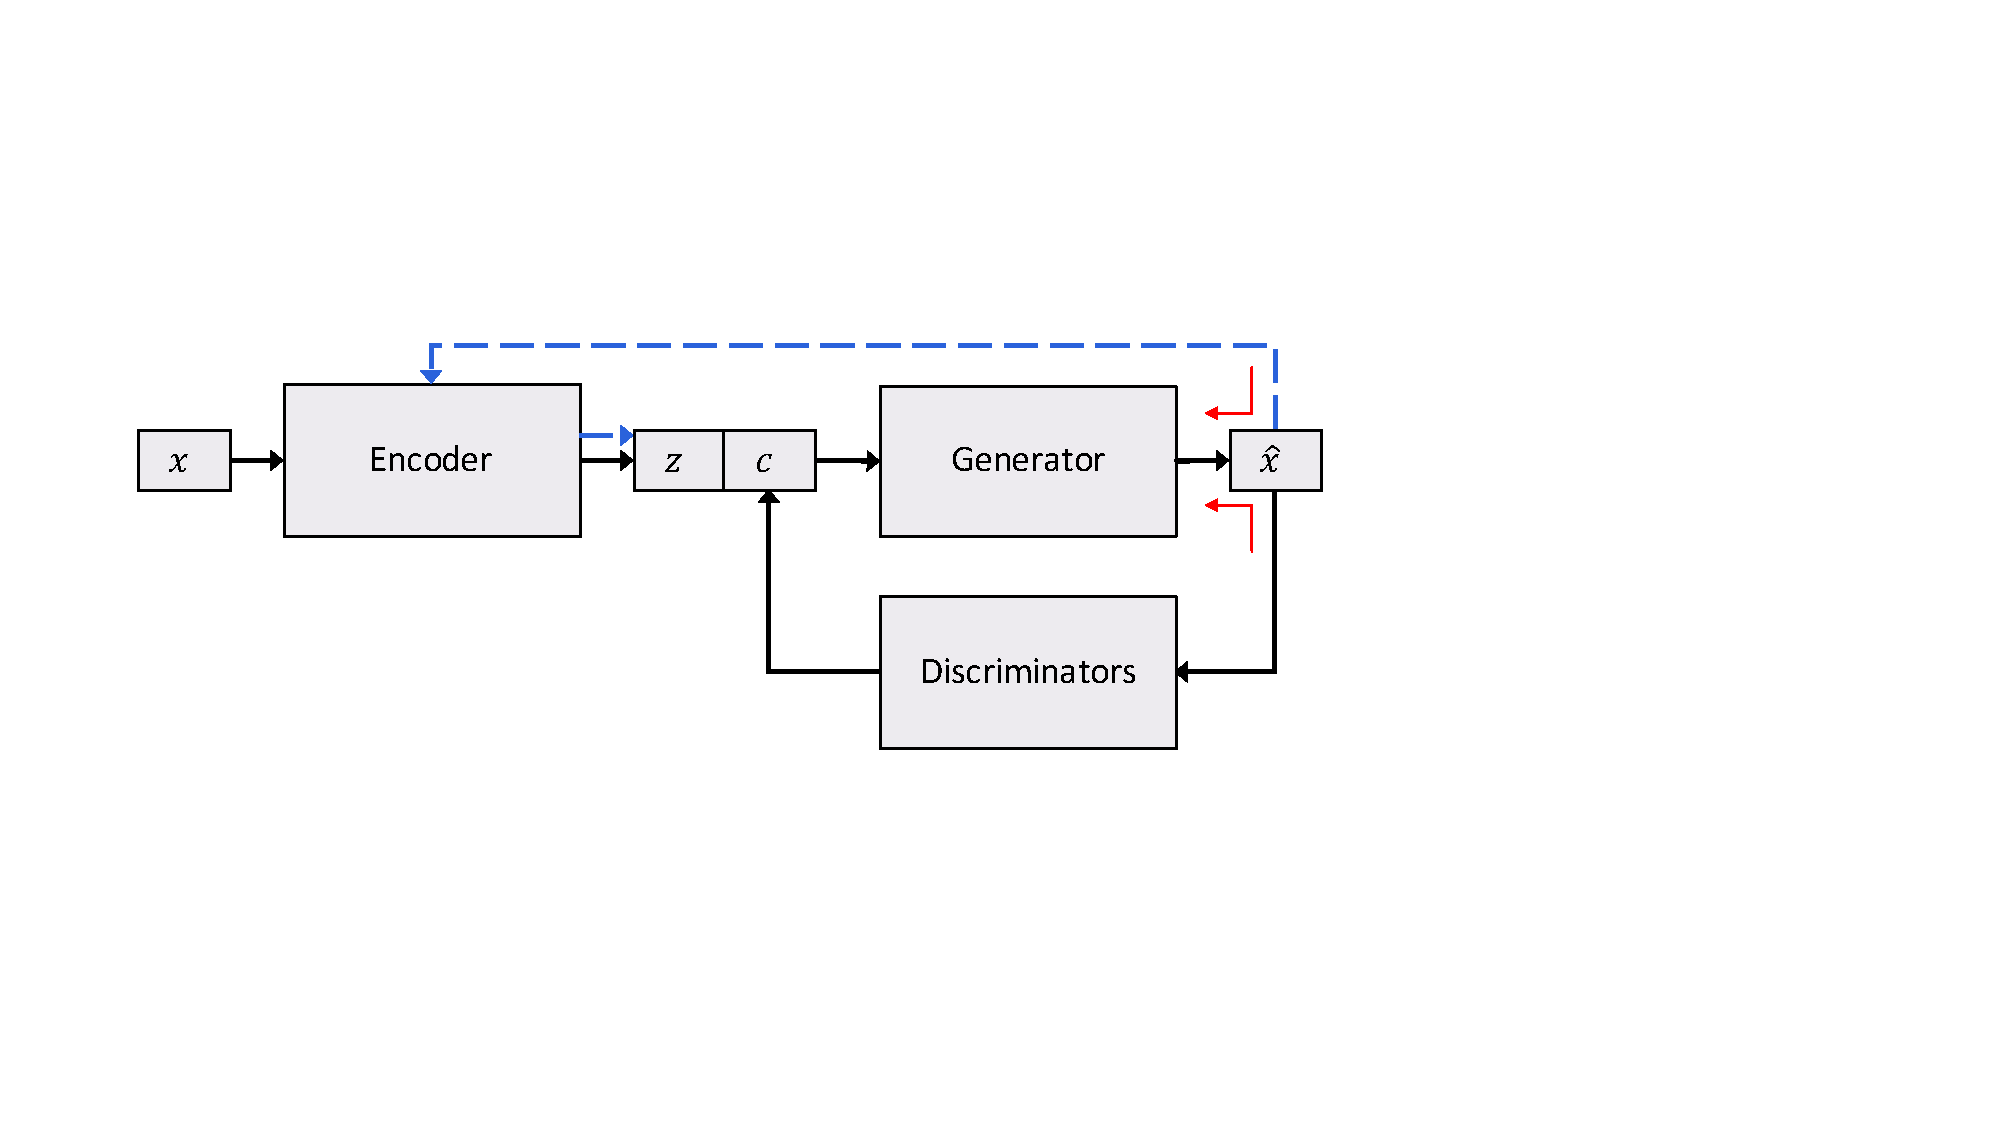
\includegraphics[width=\textwidth]{images/tcg-architecture}
	\end{figure}
	\imgsrc{\citet{hu2017toward}}
\end{frame}

\begin{frame}{Cross-Aligned Style Transfer}
	\centering
	\begin{figure}[ht]
		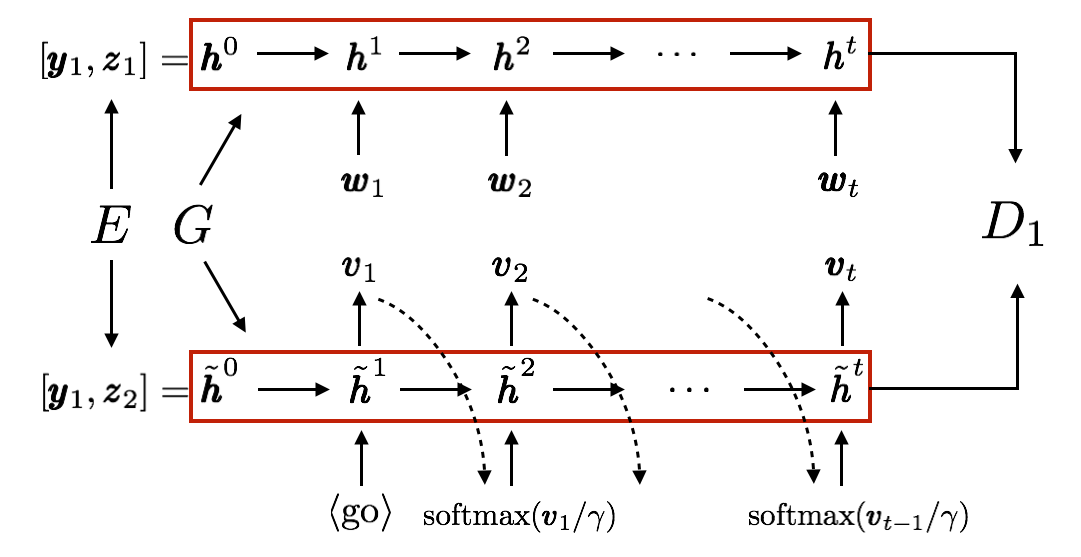
\includegraphics[width=0.9\textwidth]{images/stca-cross-align}
	\end{figure}
	\imgsrc{\citet{shen2017style}}
\end{frame}

\begin{frame}{Style Transfer using Style Embeddings and Multi-Decoders}
	\centering
	\begin{figure}[ht]
		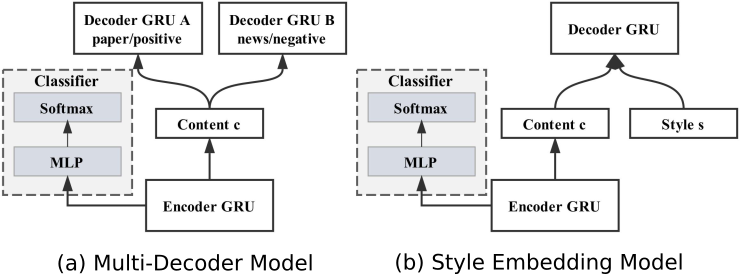
\includegraphics[width=\textwidth]{images/semb-architecture}
	\end{figure}
	\imgsrc{\citet{fu2017style}}
\end{frame}

% 

\section{Summary}

\begin{frame}{Summary}
	\begin{itemize}
		\item We describe auxiliary objectives that augment a vanilla autoencoder, including a dual-adversary setup containing a novel bag-of-words adversary.
		\item Our model generalizes to multi-class problems without requiring multiple discriminators \citep{hu2017toward,shen2017style} and multiple decoders \citep{fu2017style,prabhumoye2018style}.
		\item We show that the auxiliary objectives can separate latent variables for style and content, qualitatively and quantitatively.
		\item We apply this method to style transfer tasks in language and achieve state-of-the-art performance, without any explicit style transfer objective.
	\end{itemize}
\end{frame}

\begin{frame}[allowframebreaks]
	\bibliography{presentation}
	\bibliographystyle{unsrtnat}
\end{frame}

\begin{frame}
	\centering
	\Huge{Questions?}
\end{frame}


\end{document}
